\documentclass[]{scrreprt}
\usepackage[linesnumbered]{algorithm2e}
\usepackage{listings}
\usepackage{color}
\usepackage{graphicx}
\usepackage{subcaption}
\usepackage{mwe}
\usepackage[titletoc]{appendix}
\definecolor{dkgreen}{rgb}{0,0.6,0}
\definecolor{gray}{rgb}{0.5,0.5,0.5}
\definecolor{mauve}{rgb}{0.58,0,0.82}

\lstset{frame=tb,
	language=Java,
	aboveskip=3mm,
	belowskip=3mm,
	showstringspaces=false,
	columns=flexible,
	basicstyle={\small\ttfamily},
	numbers=none,
	numberstyle=\tiny\color{gray},
	keywordstyle=\color{blue},
	commentstyle=\color{dkgreen},
	stringstyle=\color{mauve},
	breaklines=true,
	breakatwhitespace=true,
	tabsize=3
}
\title{CmpE 483 Project 2 \\Visual Implementation of Decenteralized Lottery 
	 }
\author{Korhan \c{C}a\u{g}{\i}n Gebolo\u{g}lu - 2012400075\\Salih Sevgican -2013400219 \\Ahmet Bu\u{g}rahan Ta\c{s}dan - 2013400156\\ Group Name:ZAUM}
\date{Spring 2018}

\begin{document}
\maketitle
\cleardoublepage
\pagenumbering{roman} 
\cleardoublepage
% Let's change \thepage so it prints one less than
% the real page number; \pagenumbering{arabic}
% will redefine it to the right meaning afterwards.
\renewcommand\thepage{\romannumeral\numexpr\value{page}-1\relax}

\tableofcontents
\cleardoublepage
\pagenumbering{arabic}
\chapter{Introduction}
\section{Intro}
The aim of this project is to demonstrate how a smart contract in Solidity\cite{Solidity} can be used by any ordinary user who do not have a strong background in technology . In this course, how a smart contract can be implemented and how can we build a frontend for our contract have been covered and simply in this project, we need to code what we have learnt in this class. To be able to finish the project, we need to find a way to combine a design and our first project code. The former project was related to decentralization of autonomous lottery. To satisfy the requirements of this project, we need to implement a frontend that helps us to test our environment. We need to focus on the solving defects in first project project, design a solid web based user interface and make the connection between contract and frontend. However, before starting deep into the details of how we handled the project, to remember what is the requirements in this project would be great idea to consider. \\ 
\section{Definition}
An autonomous decentralized lottery based on smart contract which distributes specified types of tickets for a given time interval and retrieves different types of winners for this given time range and after then this, repeats the same idea next timeline. There are some requirements that must be satisfied to finish the project. This is the former project definition and this project still dependson this. In this project, we need to implement a system that helps user to play with our contract and by doing this, we build visual test environment. On the other hand, we need to use some other tools. The most significant one is Brave\cite{Brave} which is a web browser with many available resources for blockchain-based tools. The second one is a third party application that help the user to use Etherium-based blockchain system easily, which is called as Metamask\cite{Metamask}. Finally, we should be able to test our system on a network called as Ropsten Test Network\cite{Ropsten}. 


\section{Checklist}
What project expect us to do can be seperated in three part and totally 8 main specialities should be added to that system. What they are;
\begin{itemize}
	\item 
	Contract Part
	\begin{itemize}
		\item 
		Solving Defects
	\end{itemize}
	\item 
	Visualization Part
	\begin{itemize}
		\item 
		Building a User Interface
		\item 
		Connecting with contract
		\item 
		Connecting with Metamask
	\end{itemize}
	\item 
	Testing Part
	\begin{itemize}
		\item 
		Controlling contract with Ropsten
	\end{itemize}
\end{itemize}
\section{How to Run}
To run the project , you should have installed nodejs, 'web3' library and 'express' by using npm. You can install web3 1.0 version however our metamask is using web3 0.2. When you have installed required dependencies in the project folder type 'node myserver.js'. Then in your metamask installed browser (Connected to Ropsten test net), open remix solidity first, deploy Lottery.sol file to ropsten network, allow transaction through metamask , then wait for deployment. After deployment, copy abi and paste it under index.html, to 'test\_abi' variable, do the same for deployment address, paste deployment address to 'test\_address' variable. 
Lastly, from your browser enter the URL: localhost:8081/index.html , now you're ready to test.
	
	\chapter{Contract Part}
	Contract Part is the base implementation part of the project and in this part, we need to build a structure for this project. We need to build a smart contract that allows users gets one or more tickets which will be used in a lottery. The user will send a number that they bet on. Our contract will calculate a big winner and some small winners. After this process, the winners gets the money and if their accounts eligable to withdraw the money, they can collect their money.\\
	To be able satisfy this scenerio, we divided the coding part into four main part and one helper part. The helper part is just a bunch of functions that retrieves information about the current status of the contract. We also have some internal class level variables that helps the system to save the information about current status and the details of the buyers. The part that we classified will be elaborated more in the upcoming sections one by one. \\
	The implementation of the first project has been preserved. We were aware of some defected parts that we could not implemented. We tried to solve some of them in this project. We explained the details in the updates section.
	 \section{First Project Structure}
		\subsection{Ticket Declaration}
		The ticket structure is the milestone of the project because the transaction resulted with creating a ticket depends on the how many gas sent by the buyer and with this ticket buyer will join the lottery to win the prize. One ticket consists of four different elements. All of them stores one significant feature of the ticket.  \\
		The first item of the ticket is tip and it is the declaration of what kind of ticket this ticket is. This information helps the system to calculate how big the prize will be because there are three different types of ticket and the reward is diferantiated by this element. \\
		The next item is related to who sent this gas to get the ticket. It basically stores the sender's hash address in the ticket. It will speed up the validation process of ticket and check whether this ticket is winner or not.\\
		N is used in the revealing phase. It is sent by the buyer and used for the correctness of ticket. \\
		The last item is the declaration of whether this ticket validated or not.
		\subsection{Purchasing}
			We start with controlling with the incoming gas size. If it acceptable, we proceed to create ticket. After creating the ticket, we store the ticket in the contract due to use that information at the revealing phase. Our algoritm can be described like below.
			\begin{algorithm}[H]
				take(val) from sender\\
				get(tickets) from system\\
					\eIf{msg.value!=8 finney and\\ 
						msg.value!=4 finney and \\
						msg.value!=2 finney}{
						revert();\\
					}{
					$ticket \longleftarrow createTicket() $\\
						\If{msg.value==8 finney}{
							$ticket.tip \longleftarrow 1 $\\
						}
						\If{msg.value==4 finney}{
							$ticket.tip \longleftarrow 2 $\\
						}
						\If{msg.value==2 finney}{
							$ticket.tip \longleftarrow 3 $\\
						}
						
						$ticket.ticket_hash\longleftarrow val $\\
						tickets.push($ticket$)\\
					}
			\end{algorithm}
		\subsection{Revealing}
		This function takes ticket number as parameter. If an address has bought more than one ticket, than they have to reveal their numbers by order. For example if an address has sent a hash code(purchase) by using Ticket number 12 and 24, then it has to reveal its tickets by sending first 12 then 24. Reveal function also checks whether it is the last block of the lottery or not, if it is, then it maps winner numbers address for reimbursment according to Ticket type. If it is not the last block then it checks number with the hash code which is send in purchase function, if it checks out then winner number is XOR'ed with the given parameter. If it is not a valid ticket then winner number is not XOR'ed with the parameter.
		\subsection{Withdrawing}
		In the revealing phase if a ticket owner gains a right to withdraw, reimbursement map in the code has the address and the amount of gas that needs to be sent. If sender's ticket number has won the lottery then withdraw function returns required amount of money. 
	 \section{Updates}
	 	Unlike the first project now we hold the count of lotteries. All the lottery money now is seperated, when a lottery revealed, the winner can withdraw money gathered in that lottery's purchase phase. In this project, you should copy and paste ABI and contract deployment address into index.html file in 'test\_abi' and 'test\_address'.
	\chapter{Visualization Part}
		There are many options in the market for creating a beautiful web sides. We had to choose one of them for this project. We started with investigating React\cite{React} which is javascript-based web and mobile cross platform. We could use this but it seems to be a waste of time. That's why, we choose a simple and useful bootstrap structure for this project which provides an elegant user interface for user. For this project, we combined two example view that can be founded in github and we just took it and customised options the way that we need to. We successfully finished this part. 
		\subsection{Customisation}
		The first view example we owned can be founded in here\cite{1}. This is the basic structure for our visualization. We used custom div elements to create those side by side views for getter methods.\\
		The problem in the first example is that it is not useful for a textareas. We used another example to complete the view example, link can be founded in here\cite{2}. With adding this one, we finished visualization for our web interface.
				\begin{figure}[h!]
					\centering
					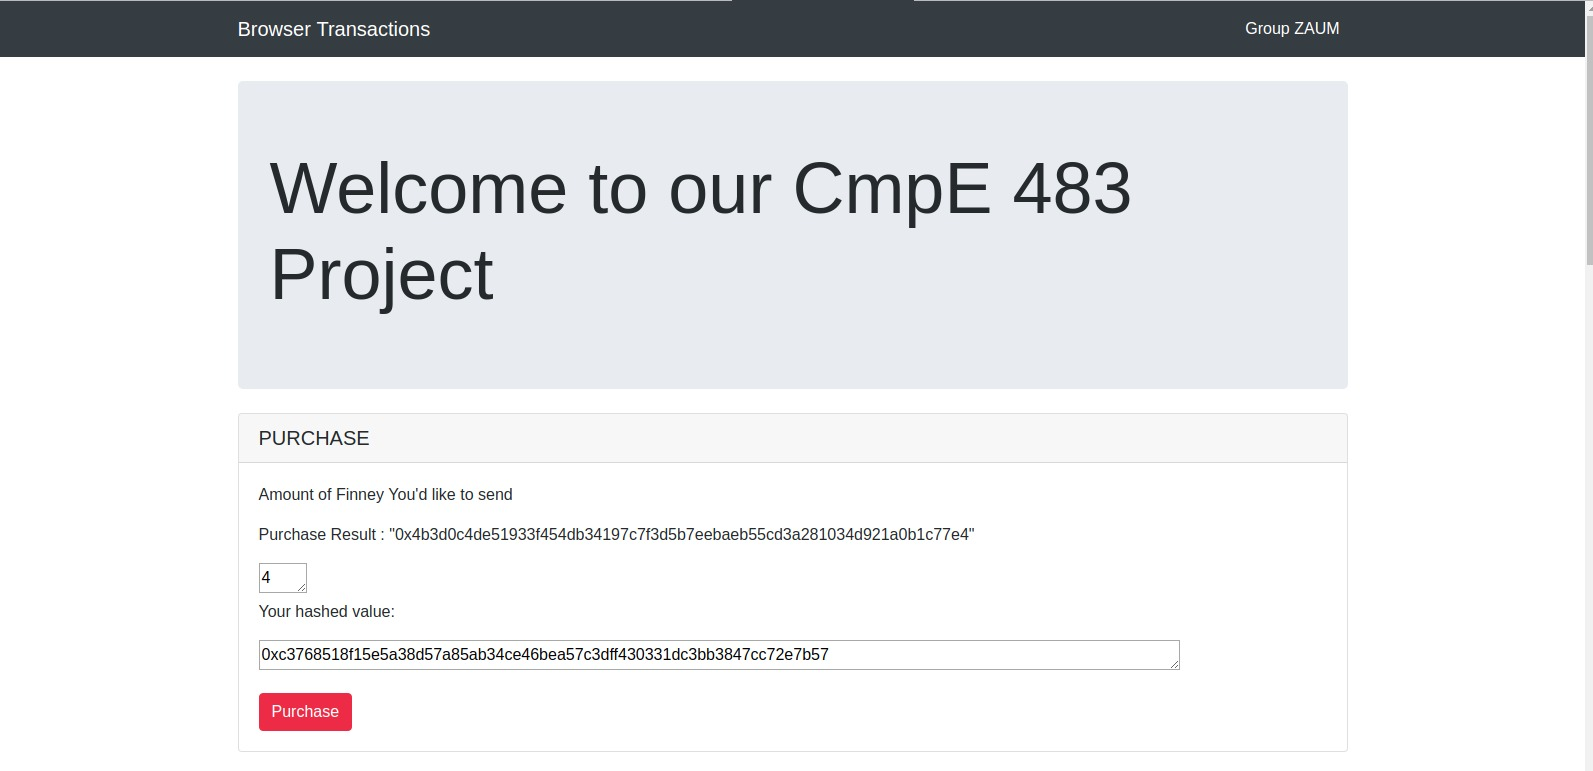
\includegraphics[scale=0.28]{12.jpeg}
					\caption{Screenshot of web interface 1}
				\end{figure}
					\begin{figure}[h!]
						\centering
						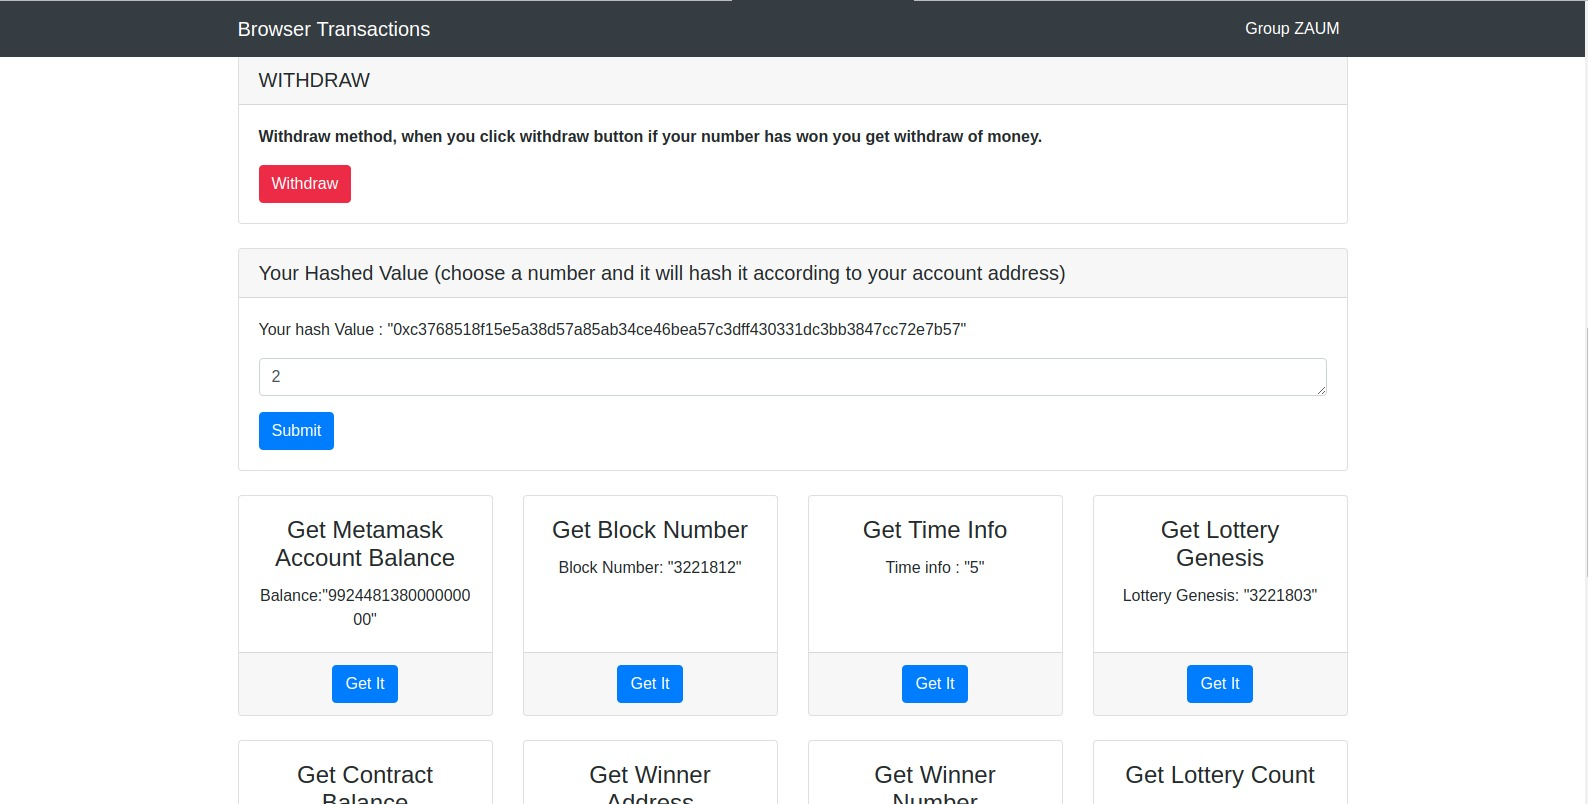
\includegraphics[scale=0.24]{11.jpeg}
						\caption{Screenshot of web interface 2}
					\end{figure}
		\subsection{Connections}
		We used the lab examples and we embed a javascript code directly into our single page html called as metamask.html. We connect this script with our view components by using basic structure of html. We give spesific id for every changeable component and manipulate these component by using id.

\chapter{Testing Part}
		We tested our contract with different cases. We need to see the lottery can be finished and the transaction can be complited. We used the same logic with the first project.
		\subsection{Create Different accounts}
		The contract is meaningless without users. That's why, we need to add new users that can play with our lottery contract. User are capable to buy three different types of tickets according to the gas they sent. We created four different accounts in order to use in our testbed. We also add the private informations of the accounts into the test code due to be able use in it.
		\subsection{Purchase the tickets}
		The accounts can buy the tickets in different amounts and buys more than one ticket for turn. We wrote  those in different orders to be able to see different results. 
		\subsection{Sending the money}
		After the revealing results, we are just checking the accounts in order to display the account's balances change. 
		\subsection{Distributability of Prize}
		The system can run for different times and accounts can win the prize according to what they sent to system.
\chapter{Assessment and Conclusion}
In this project, we need to have an Ethereum identity that the our local website can recognize and interact with. To achive this,  MetaMask extension is the best option to implement that project can be coded on. Although it is suitable to use in the project, the concept that we are getting familiar with is hard to process and understand. However, the best practise we can get is playing with these tools. That's why what we tried to do in this procect is helpful.\\
We are successfully implemented building a web-based user interface for the our Lottery Contract. Our website is working perfectly by itself. Our old contract has some missing parts. We have successfully finish the incomplete parts. We wish to develop a fully functional Contract \\
On the other hand, our contract is not distributing the second and third winner but it can be added to the system easily.\\
The overall results of the project is better than our expectations. The web-based user interface for our Lottery smart contract works perfectly.


\begin{appendices}


\end{appendices}

\begin{thebibliography}{9}

	\bibitem{JavaScript} 
		JavaScript,
		\\\texttt{https://developer.mozilla.org/bm/docs/Web/JavaScript/}
	\bibitem{Solidity} 
		Solidity Language version.0.4.23,
		\\\texttt{https://solidity.readthedocs.io/en/v0.4.23/}
	\bibitem{Brave} 
		Brave Browser,
		\\\texttt{https://brave.com}
	\bibitem{Metamask} 
		Metamask ,
		\\\texttt{https://metamask.io}
	\bibitem{Ropsten} 
			Ropsten , 
			\\\texttt{https://ropsten.etherscan.io}
	\bibitem{React} 
	React.js , 
	\\\texttt{https://reactjs.org}
	\bibitem{1} 
	Heroic Features , David Miller
	\\\texttt{https://github.com/BlackrockDigital/startbootstrap-heroic-features}
	\bibitem{2} 
	Blog Post ,David Miller 
	\\\texttt{https://github.com/BlackrockDigital/startbootstrap-blog-post}
			
		
\end{thebibliography}

\end{document}          
